\section{Technical limitations/complications for the optics control}

List the things that would have needed to be changed to reached better results:

\begin{itemize}
\item Stable and reliable power of of the TWTs
\item Additional signals to control the injector
\item More trustworthy BPMs
\item Possibility to double check the results from the screen (in terms of emittance)
\end{itemize}

\subsection{Stability and availability}
In a linear machine a change of the initial parameters of the beam will propagate and also change the optics parameters downstream. It is therefore important to have very good control of the injector parameter. A major issue to obtain a good factor~8 has been the availability of the TWTs as well as keeping them at the same power and phase. Many attempts to mitigate this effect has been performed through and improved reference system to keep all signals of interest. The idea was through keeping the loading and the BPR signals constant we could retrieve the same beam conditions. As a further step also beam feedbacks have been implemented to automatically mitigate this effect. However, even with these feedback in place it was not always possible to compensate since the monitored signals lack the sensitivity needed to retrieve similar beam conditions. In these cases it is then sometimes needed to redo an optimization of the injector which in turn might impact the optics and beam energy.
In some cases it might actually be impossible to get exactly the same beam conditions back after a change. Another issues is that the BPRW which are one of the most important signals for the injector feedbacks is not only dependent on the bunch length but also dependent on the position on the beam and beam current. They are in principal things that can be monitored and corrected by other devices. 

\subsection{Beam instrumentation}
The optics control is never better than the beam instrumentation. We will here try to outline some of the major issues we have experienced with the beam instrumentation in CTF3.
\subsubsection{Charging up effect for multi-turns}
One problem is the charging up effect of a certain type of BPI. This has limited the use of this type of BPM in setting up multi-turn in the CR. An example of this charging up effect is seen in figure~\ref{fig:bpi_charging_up}. The effect is not easy to remove reliable since the charging up depends on the position as well as the charge \cite{ben_constance_chargingUp}. 
\begin{figure}
\begin{center}
% 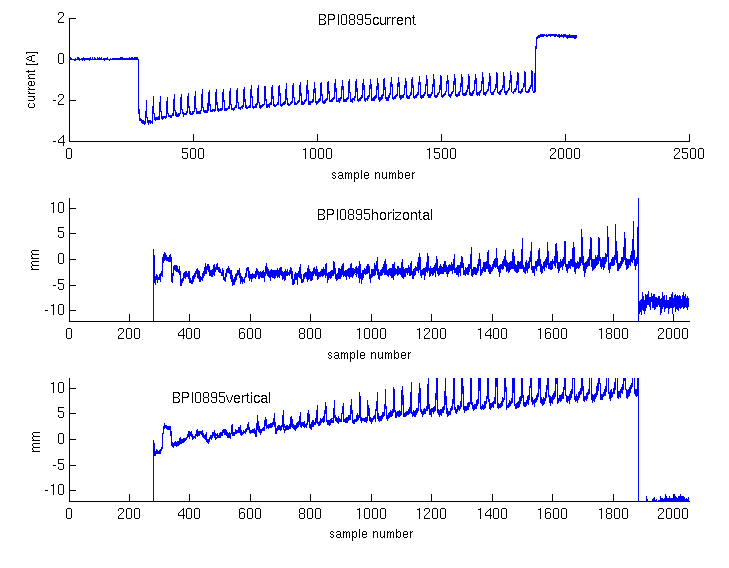
\includegraphics[width=1\linewidth,natwidth=729,natheight=568]{BPI0895.png}
 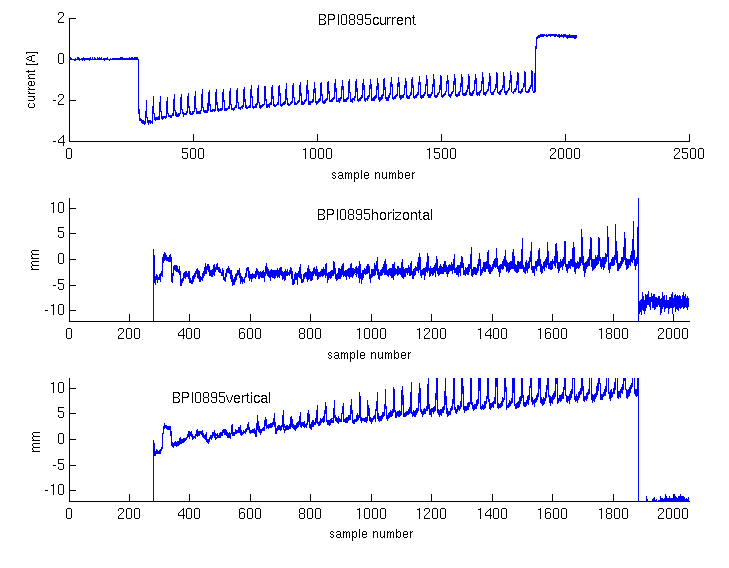
\includegraphics[width=1\linewidth]{BPI0895.png}
 \caption{}
\label{fig:bpi_charging_up}
\end{center}
\end{figure}

This is to be compared to a BPM, as seen in figure~\ref{fig:bpm_not_charging_up}, where this effect is not present in the position signal. This has limited us to the use of this types of BPMs when observing the position for many turns. 

\begin{figure}
\begin{center}
 %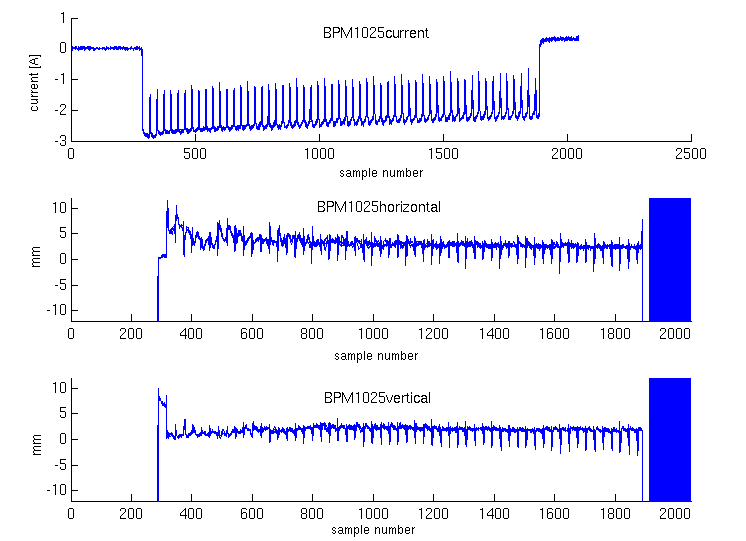
\includegraphics[width=1\linewidth,natwidth=746,natheight=541]{BPM1025.png}
 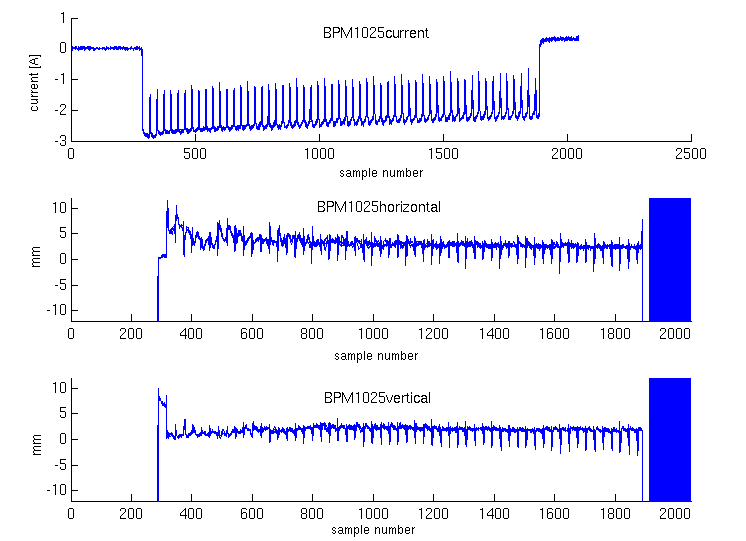
\includegraphics[width=1\linewidth]{BPM1025.png}
 \caption{BPM}
\label{fig:bpm_not_charging_up}
\end{center}
\end{figure}


\subsubsection{Frequency dependency of the BPMs \textbf{Davide}}
%\subsubsection{Orbit Closure}
%\subsubsection{Optics Closure}
\subsection{Powering \textbf{Tobias and Davide}}
\subsubsection{Common powering}
\subsubsection{Septa}

\begin{table}[]
\centering
\caption{My caption}
\label{my-label}
\begin{tabular}{lllll}
Girder & plane  & factor  & emittance &  \\
27 & H & 4  & 75-100  &  \\ \hline
27& V  & 4 & ? &  \\ \hline
27& H & 8 & 245 &  \\ \hline
27& V & 8 & 110 &  \\ \hline
30 & H & 4  & 173  &  \\ \hline
30& V  & 4 & 96 &  \\ \hline
30& H & 8 & 467 &  \\ \hline
30& V & 8 & 149 &  \\ \hline

\end{tabular}
\end{table}

